\subsection{Identification} \label{subsec:identification}

This subsystem takes an image classified as 'cat' by the classification subsystem and recognizes or identifies the cat in the image. This is necessary for profiling the cats and tracking their feeding logs.

\subsubsection{Requirements}

The requirements for this subsystem follow:

\begin{itemize}

\item The subsystem should be able to identify new cats.
\item The subsystem should be able to recognize identified cats.

\end{itemize}

\subsubsection{Solution}

\begin{figure}[h!]
    \centering
    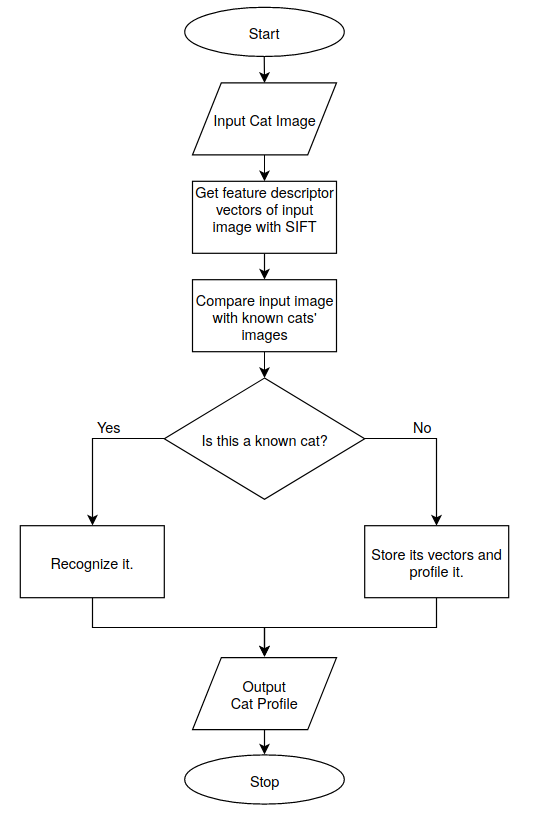
\includegraphics[width=0.55\linewidth]{img/sift_algorithm_flowchart.png}
    \caption{Algorithm Flowchart of the Identification subsystem}
    \label{fig:sift_algorithm_flowchart}
\end{figure}

For identification purposes, one of the most powerful feature detection algorithms, SIFT (Scale-Invariant Feature Transform), is used on the initial tests.

The algorithm flowchart of this subsystem is in Figure~\ref{fig:sift_algorithm_flowchart}. The subsystem starts with an image input. Since this image is fed from the classification subsystem, it is certainly an image of a cat. Later, this image's feature descriptor vectors are obtained by SIFT and compared to the stored vectors of images of known cats. This comparison is the most crucial part of the entire process; most of the past and future tests of this subsystem will have been done on various methods of comparing these vectors. After this vector comparison, if any known cat's features are similar enough, it is decided that the input cat image belongs to that cat. Otherwise, the cat is identified as a new cat, and a new profile for it is set up. Lastly, the cat's profile is returned as the output of the subsystem, and the process ends.

Figure~\ref{fig:sift_example} is an example of the SIFT key feature extraction. The image on the right is a mapping of the features on the original image of our beloved friend Ponçik on the left.

\begin{figure}[h!]
    \centering
    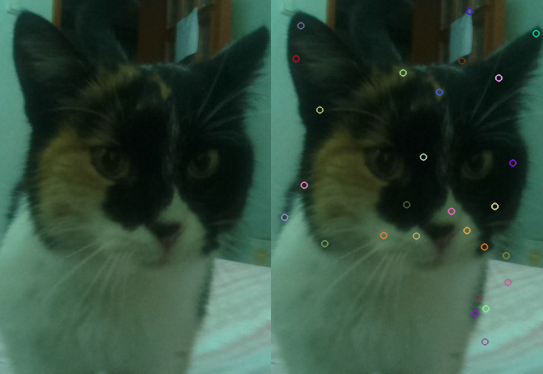
\includegraphics[width=0.8\linewidth]{img/sift_example.png}
    \caption{SIFT feature mapping}
    \label{fig:sift_example}
\end{figure}

Current implementation of vector comparison computes a loss between two vectors. This loss is simply the euclidean distance between the two vectors:

For vectors x and y with n elements each:
\begin{equation}
    d = \sqrt{(x_{1}-y_{1})^{2}+(x_{2}-y_{2})^{2}+(x_{3}-y_{3})^{2}+...+(x_{n}-y_{n})^{2}}
\end{equation}

During a comparison of the input image with one of the stored images, each input vector is compared with all vectors of the stored image, then the smallest euclidean distance is saved as that vector's loss. Then all input vectors' losses are summed together to yield the loss between those two images. When this loss falls below the defined threshold, the input image is matched with the compared stored image. This is the case of recognition of known cats. When the loss of the input image against any stored image is larger than the threshold, the vectors of the input image are saved, and a new profile is set up for the unrecognized cat.

\subsubsection{Risks}

% ===== Indicate alternative solutions ===== %
The problem with comparing images using euclidean distances of vectors is that the loss values are not self normalized. One alternative is to use the cosine of the angle between said vectors. This method ensures that the loss values are always between 0 and 1, which results in a more coherent identification module. Nonetheless, using the euclidean distance of the vectors is preferred over using their angles with respect to each other. The reason for this is that vectors consist of both magnitudes and angles, and magnitude is anticipated to play a larger role in the case of SIFT vectors.

Aside from SIFT, there are some other feature detection algorithms that are being considered by the Computer Vision team. These include, but are not limited to, SURF (Speeded-Up Robust Features), Harris Corner Detector, FAST (Features from Accelerated Segment Test) and ORB (Oriented FAST and Rotated BRIEF).

\subsubsection{Tests}

This subsystem is currently ahead of schedule. Hence, it is not the priority of the team; consequently, there has not been considerable amounts of tests.

\subsubsection{Plans}

Future plans of this subsystem follow.

\begin{itemize}
    \item Decide on a feature detection algorithm. Some possible choices are SIFT, SURF, FAST, ORB, and Harris Corner Detector.
    \item Decide on an image comparison method that detects whether the input image belongs to a known cat.
\end{itemize}

From the Computer Vision team, Furkan is responsible for the future work regarding this subsystem.

\subsubsection{Anticipated Difficulties}

Since interfering with the way SIFT extracts the feature vectors is not an option, there is no guarantee that the extracted vectors will always be helpful. If this turns out to be an issue for the overall system, the team will consider doing background research to use another feature extraction algorithm that is more customizable.

\subsubsection{Test Plans}

Future plans on how this subsystem will be tested are listed below:

\begin{itemize}
    \item Images of various cats will be stored.
    \item These will be labeled either as 'known' or 'unknown', arbitrarily.
    \item Cats with the label of 'known' will be fed into the algorithm.
    \item Cats with the label of 'unknown' will separately be fed into the algorithm.
    \item Input image of any label will be compared with 'known' cat images.
\end{itemize}

There are two criteria for a successful test result:

\begin{enumerate}
    \item When a 'known' cat's image is fed into the algorithm, the algorithm recognizes that cat.
    \item When an 'unknown' cat's image is fed into the algorithm, the algorithm identifies it as a new cat and sets up a new profile for it.
\end{enumerate}

% ===== Measure of success ===== %